\documentclass[../main.tex]{subfiles}
\begin{document}

%% convention is base space \times fiber bundle
%% change B to K
\section{Notation \& Definitions}

%% give the why of the math after every mention of why
 
In this section we introduce a mathematical description of the visualization pipeline where artist $\mathscr{A}$ functions transform data space $\mathscr{E}$ to an intermediate representation in a prerendered graphic space $\mathscr{H}$. 

\begin{equation}
    \label{eq:artist}
    \mathscr{A}: \mathscr{E} \rightarrow \mathscr{H}
\end{equation}

We use fiber bundles\cite{FiberBundle2020, rowlandFiberBundle} to model data and graphics because they allow us to seperate the fields in a dataset from how the values in those fields are connected to each other:
\begin{itemize}
\item $E$ is a locally trivial fiber bundle over $K$ representing data space.
\item $H$ is a fiber bundle over $S$ representing visual space
\item $K$ and $S$ are a triangulizable topological space or a CW complex encoding the connectivity of points in $E$ and $H$ respectively
\end{itemize}

The fiber bundles mentioned in this work are assumed to be locally trivial\cite{spanier1989algebraic,LocallyTrivialFibre}. 


\subsection{Data Space}
As proposed by Butler \cite{butlerVectorBundleClassesForm1992,butlerVisualizationModelBased1989}, we model data as a fiber bundle ($E$, $K$, $\pi$, $F$)

\begin{equation}
    \label{eq:fiber_bundle}
    \begin{tikzcd}
        F \arrow[r, hook] & E \arrow[r, "\pi"] & K
    \end{tikzcd}
\end{equation}

with topological total space $E$, base space $K$, fiber space $F$, and the map from total space to base space $\pi: E \rightarrow K$. Maps from $K$ to $E$ are called sections and select specific points in $K$. The global space of sections in $E$ is $\Gamma(E)$.

\subsubsection{Base Space $\mathcal{K}$}
\label{sec:base_data}
\begin{figure}[H]
    \includegraphics[width=\textwidth]{figures/sections/math/k_different_types.png}
    \label{fig:base_space_types}
    \caption{The topological base space $K$ encodes the connectivity of the data space, for example if the data is independent points or a map or on a sphere}
\end{figure}

Datasets have a semantic topology such as the values are interpreted as discrete observations or part of a timeseries or map, or nodes in a networks \cite{munznerWhatDataAbstraction2014,geveci2012vtk}. As illustrated in fig~\ref{fig:base_space_div}, $K$ is this underlying structure. $K$ does not directly know the values; instead it is the sections that define the lookup between keys $k \in K$ and the corresponding values in $E$.


\begin{figure}[H]
    \label{fig:base_space_div}
    \includegraphics[width=.5\linewidth]{figures/sections/math/k_qspace.png}
    %%include second figure where fiber goes otherway
\end{figure}
The topology $K$ and the fields $F$ are determined by how $E$ is subdivided\cite{QuotientSpaceTopology2020,QuotientSpaceTopology2020}. In figure~\ref{fig:base_space_div} we can divide a rectangular base space such that there is a short fiber and long base space or a long fiber and short base space. This is analogous to long and wide forms of the same table \cite{wickham2014tidy}.

\paragraph{Triangulization}
\label{sec:triangulization}

The base space $K$ is a representation of the connectivity of the data, specifically whether the points in $E$ are discrete or sampled from a continous space. The same dataset can be expressed with different $K$. 

In our draft implementation of the data as fiber bundle model, we represent $K$ as a simplacial complex. 

\begin{figure}[H]
    \label{fig:simplex}
    \includegraphics{figures/sections/math/simplex.png}
    \caption{Simplices encode the connectivity of the data, from fully disconnected (0 simplex) observations to all observations are connected to at least 3 other observations. Higher order simplicies are outside the scope of this paper.}
\end{figure}

K is a triangularizable topological space; one triangularization scheme is as a set composed of simplices, such as those shown in figure~\ref{fig:simplex}. 


\subparagraph{Example}
chopping up a torus maybe? talk about how that gets unpacked into triangles and then into vertices


\subsubsection{Fiber Space}
\label{sec:fiber_data}

%% pull fiber stuff up here? what is it? why? fiber as cartesian product of sets
%% actual values are in the fiber 
%% gonna view spaces as simple piece put together 
%% Our fibers are cross products of (column name, domain) as described by Spivak's \cite{spivakSIMPLICIALDATABASES}. 


\begin{equation}
    \label{eq:fiber_local_trivial}
    \begin{tikzcd}
        \pi^{-1}(U) \arrow[r, "\varphi"] \arrow[d, "\pi"'] & U \times F \arrow[ld, "\mathrm{proj}_U"] \\
        U                                                  &                                         
    \end{tikzcd}
\end{equation}
such that $\varphi: \pi^{-1}(U) \rightarrow U \times F$ is a homeomorphism where $\pi$ and $\mathrm{proj}_U$ both map to $U$ and the fiber over $k$

%% rewrite this section - what are the goals here and why should we care? 
%% devoid of any context

$F_k = \pi^{-1}({k}) $ is homomorphic to the fiber $F$.
%% add a sentence for why we care
%% fibers are cartesian products of these typles sets (name, domain, monoidal action) 

%%the break out more about how fibers are cross products and what that means and how that's the structure - pull the monoids definitions here 

\paragraph{Definition}
A monoid\cite{Monoid2021} $M$ is a set that is closed under an associative binary operator $\ast$ and has an identity element $e\in M$ such that $e\ast a= a \ast e = a$ for all $a \in M$. A left monoid action \cite{SemigroupAction2021,ActionNLab} of $M$ is a set $X$ with an action $\bullet$ with the properties:
\begin{description}
    \item[closure] $\bullet: M\times X \rightarrow X$,
    \item[associativity] $\text{for all } m,t \in M \text{ and } x\in X, m\bullet(t\bullet x) = (m\bullet t) \bullet x$
    \item[identity] $\text{for all } x\in X, e\in M,  e\bullet x = x$ 
\end{description} 


$M = M_{1} \times M_{2} \times \ldots \times M_{n}$

\paragraph{Example}
%% stevens scales are examples of this 
%% one ecample of F1 is (names, strings, concat), (ordinal, Z,  ordering), () 



\subsubsection{Section}
\label{sec:section_data}
%% add context
The section $\tau$ is the mapping from base space to total space $\tau: K\rightarrow E$ 
\begin{equation}
    \label{eq:section}
    \begin{tikzcd}
        F \arrow[r, hook] & E \arrow[d, "\pi"']           \\
        & B \arrow[u, "f"', bend right]
    \end{tikzcd}
\end{equation}

such that $f$ is the right inverse of $\pi$
\begin{equation}
    \label{eq:section_domain}
    \pi(f(k)) = k \text{ for all } k \in K 
\end{equation}

In a trivial fiber bundle, $E = K \times F$ \cite{rowlandFiberBundle,FiberBundle2020}:
\begin{equation}
    \label{eq:section_return}
f(b) = (b, g(b))
\end{equation}

where the domain of $g(b)$ is $F_b$ and returns a point $p$ in $F_b$. The space of all possible sections $f$ of $E$ is $\Gamma(E)$. All sections $f \in \Gamma(E)$ have the same fibers $F$ and connectivity $K$. 
\paragraph{Example}
%%talk about table and all that jazz

For each field $c \in C$, the record function $r: C \rightarrow U_{\sigma}$ returns an object of type $\sigma(c) \in DT$. The set of all records $\Gamma(\sigma)$ is the set of all sections on $U_\sigma$. Spivak defines the $\tau$ mapping from an index of databases $K$ to records $\Gamma(\sigma)$ as $\tau: K \rightarrow \Gamma(\sigma)$. This is equivalent to $\tau: k \rightarrow E$ since $F = \Gamma(\sigma)$ and $F$ is the embedding in $E$ on which the records $r$ lie.
 

\subsubsection{Sheaf and Stalk}

Often a graphic may need to be updated with live data or support zooming in on a segement of the dataset; to support working with a subset of data, we can use the sheaf $\mathcal{O}(E)$

\begin{equation}
    \label{eq:sheaf}
    \begin{tikzcd}
        \iota^*E \arrow[d, "\pi"']           & E \arrow[d, "\pi"'] \arrow[l, "\iota^*"']         \\
        U \arrow[u, "\iota^*\tau"', bend right] & K \arrow[u, "\tau"', bend right] \arrow[l, "\iota"']
        \end{tikzcd}
\end{equation}
which is the localized section of fibers $\iota^*\tau: U \rightarrow \iota^*E$ pulled back via the inclusion map $\iota: U \rightarrow K$. The localized section is the germ $\xi^*\tau$. The neighborhood of points $k_i$ surrounding the point $k$ the sheaf lies over is the stalk $\mathcal{F}_b$ \cite{StalkSheaf2019,spanier1989algebraic}.

The jet bundle $\mathcal{J}$ \cite{JetBundle2020,musilovaCalculusVariationsJet2016} is a type of sheaf that allows for writing differential equations on sections of fiber bundles; this information is required for some visual characteristics, such as line thickness. 

\subsubsection{Example: Temperature}
\textcolor{red}{Moved \& walked through b/c was getting clunky to not have terms yet}\\
The fiber bundle model is flexible enough to express some of the many different forms that temperature data can come in. 

\begin{figure}[H]
    \begin{subfigure}{.5\textwidth}
        \includegraphics[width=\textwidth]{figures/sections/math/temp_1k.png}
        %% add box around neighboring P and Map
        \label{fig:base_example_line}
    \end{subfigure}
    \begin{subfigure}{.5\textwidth}
        \includegraphics[width=\textwidth]{figures/sections/math/temp_2k.png}
        \label{fig:base_example_plane}
    \end{subfigure}
    \label{fig:base_example}
    \caption{These two datasets have the same fiber of temperature but different base spaces. In figure~\ref{fig:base_example_line} the temperature values are 1D continuous, while in figure~\ref{fig:base_example_plane} the temperature values are 2D continuous.}
\end{figure}

The datasets in figure~\ref{fig:base_example} have identical fibers that encode a set of temperature values. In figure~\ref{fig:base_example_line} the temperatures lie on a line such that a section could return a timeseries or a distribution. In figure~\ref{fig:base_example_plane}, the temperatures lie on a 2D continuous plane; a section could return a map or contour. Because the fiber is 1D, it does not encode metadata 

\begin{figure}[H]
    \begin{subfigure}{.5\textwidth}
        \includegraphics[width=\textwidth]{figures/sections/math/temp_2f.png}
        \label{fig:fiber_example_plane}
    \end{subfigure}
    \begin{subfigure}{.5\textwidth}
        \includegraphics[width=\textwidth]{figures/sections/math/temp_3f.png}
        \label{fig:fiber_example_cube}
    \end{subfigure}
    \label{fig:fiber_example}
    \caption{The fiber is expanded to include metadata fields that describe the semantics of $K$. In figure~\ref{fig:fiber_example_plane} the fiber is \textrm{temperature} $\times$ \textrm{time} and in figure~\ref{fig:fiber_example_cube} the fiber is \textrm{temperature}$\times$ \textrm{latitude} $\times$ {longitude}}.
\end{figure}

To encode the metadata, the fiber is expanded as illustrated in figure~\ref{fig:fiber_example}. The fiber in figure~\ref{fig:fiber_example_plane} is the cartesian product of the space of possible temperature values in degrees celsius and space of possible time values
\begin{equation}
F = [temp_{min}, temp_{max}] \times [time_{min}, time_{max}]
\label{eq:fiber_plane}
\end{equation}

while the fiber in figure~\ref{fig:fiber_example_cube} is the cartesian product of temperature, latitude, and longitude
\begin{equation}
F = [temp_{min}, temp_{max}] \times [-90, 90] \times [-180, 180]
\label{eg:fiber_cube}
\end{equation}

such that $E$ is the space of all possible points in $F$.

\begin{figure}[H]
    \includegraphics[width=1\linewidth]{figures/sections/math/fiberbundle.png}
    \label{fig:fiber_example_section}
    \caption{The section $\tau_1$ returns the blue points,  while $\tau_2$ returns the purple points. $\Gamma(E)$ is the set of all sections, including $\tau_1$ and $\tau_2$}.  
\end{figure}
Given the fiber described in equation~\ref{eq:fiber_plane}, the sections $\tau_{1}$ and $\tau_{2}$ in figure~\ref{fig:fiber_example_section} return tuples of the form
\begin{equation}
\tau(k) = (k, (temperature, time))
\end{equation}
such that sections with the constraint that time is monotonic return a timeseries. 


\subsection{Prerender Space $H$}
\label{sec:display}
We define a graphic space $H$ such that we do not have to assume the physical output space of the renderer. This means that the graphic in $H$ can be output to a screen or 3D printed space or a dome. 

We model the prerender space as a fiber bundle (H, S, $\pi$, D). $H$ is the predisplay space, with a fiber $D$ dependent on the target display and a base space of $S$. 

\subsubsection{Base space}
The underlying topology $S$ of a graphic often needs more dimensions than the data topology $K$ because of the specifications of the display space. For example, a line plot on a plane (such as a screen or a piece of paper) by necessity needs to also have a thickness so that it is visible, which maps back to a set of connected points in $H$. The topology of these connected points is therefore the region $s \subset S$ such that $\xi: S \rightarrow K$ is a deformation retraction \cite{RetractionTopology2020}
\begin{equation}
    \begin{tikzcd}
        E \arrow[d, "\pi"'] & H \arrow[d, "\pi"'] \\
        K                   & S \arrow[l, "\xi"']
        \end{tikzcd}
\end{equation}

that goes from a region $s \in S_{k}$ to its associated point $k$, such that when $\xi(s) = k$, $\xi^*\tau(s) = \tau(k)$. 

\subsubsection{Fiber and Section}
A section $\rho: S \rightarrow H$ is a mapping from a region $s$ on a mathematical encoding of the image to a region $xy$ on the screen that the renderer then maps to visual space as defined in D.

\paragraph{Example}
For a physical screen display, we can consider a predisplay space that is a trivial fiber bundle $H=\mathbb{R}^{5}\times S$ such that $\rho$ is
\begin{equation}
    \rho(s)  = [x(s), y(s), r(s), g(s), b(s)]
    \label{eq:rho}
\end{equation}

To draw an image, a region, $H$ is inverse mapped into a region $s \in S$ where
\begin{equation}
s = \rho^{-1}_{\tiny{XY}}(xy)
\end{equation}
such that the rest of the fields in $\mathbb{R}^{7}$ are then integrated over $s$ to yield the remaining fields:
\begin{align}
    r &= \iint\limits_s \rho_{\tiny{R}}(s)ds^{2}\\
    g &= \iint\limits_s \rho_{\tiny{G}}(s)ds^{2}\\
    b &= \iint\limits_s \rho_{\tiny{B}}(s)ds^{2}
\end{align}

Here we assume a single opaque 2D image such that the $z$ and $alpha$ fields can be omitted. To support overplotting and transparency, we can consider $D=R^{7}$

\subsubsection{{Example}}
\begin{figure}[H]
    \includegraphics[width=.4\linewidth]{figures/sections/math/render.png}
    \caption{}
    \label{fig:render}
\end{figure}

As illustrated in figure~\ref{fig:render}, words.

\subsection{Artist}


In this section we will define the artist as a mapping from a sheaf $\mathcal{O}(E)$  to $\mathcal{O}(H)$. 
\begin{equation}
    A: \mathcal{O}(E) \rightarrow \mathcal{O}(H)
\end{equation}

The artist decomposes to mapping data to visual $\nu:E\rightarrow V$, then  compositing $V$ pulled back along $\xi$ to $\xi^*V$ to a visual mark in prerender space $Q:\xi^*V\rightarrow H$. 

\begin{equation}
    \label{eq:artist}
    \begin{tikzcd}
        E \arrow[r, "\nu"] \arrow[rd, "\pi"'] & V \arrow[d, "\pi"] & \xi^*V \arrow[r, "Q"] \arrow[d, "\xi^*\pi"'] \arrow[l, "\xi^*"'] & H \arrow[ld, "\pi"] \\
                                              & K                  & S \arrow[l, "\xi"']                                              &                    
        \end{tikzcd}
\end{equation}
The pullback map $\xi^*$ copies each value in $V$ over $k$ to $s$ in corresponding $S_k$ such that $\xi^*V$ can have multiple values that map to one value in $V$. 

The visual fiber bundle ($V$, $K$, $\pi$, $P$) has section $\mu: V \rightarrow K$ that resolves to a visual variable \cite{bertinIIPropertiesGraphic2011,munznerMarksChannels,} in fiber $P$. The visual transformer $\nu$ is a set of functions each targeting a different $\mu$
\begin{equation}
    \label{eq:nu_expanded}
    \{\nu_{0}, \ldots, \nu_{n}\}: \{\tau_{0}, \ldots, \tau_{n}\} \mapsto \{\mu_{0}, \ldots, \mu_{n}\}
\end{equation}

where $\mu_{i}$ are the visual parameters in the assembly function $Q(\mu_{0}, \ldots, \mu_{n})(s) = \rho(s)$. 


\subsubsection {Example: Matplotlib Visual Fiber}
For example, for Matplotlib \cite{hunterMatplotlib2DGraphics2007}, some of the possible types in $P$ are:
\begin{table}[ht]
    \label{tab:mpl_visual_variable_fiber}
    \renewcommand{\arraystretch}{2}
    \begin{tabulary}{\textwidth}{|l|L|l|}\hline
     $\bm{\nu_{i}}$                      & $\bm{\mu_{i}}$                                                            & $\bm{codomain(\nu_{i})}$  \\ \hline                                              
    position                    & x, y, z, theta, r                                                          & $\mathbb{R}$   \\ \hline
    size                        & linewidth, markersize                                            & $\mathbb{R}^{+}$   \\ \hline
    shape                       & markerstyle                                                      & $\{f_{0}, \ldots, f_{n}\}$ \\ \hline
    color                       & color, facecolor, markerfacecolor, edgecolor  & $\mathbb{R}^{4}$ \\ \hline
    \multirow{2}{*}{texture}    & hatch                                                            & $\mathbb{N}^{10}$\\\cline{2-3}
                                & linestyle                                                        & $\{f_{0}, \ldots, f_{n}\} \times (\mathbb{R}, \mathbb{R^+}^{n, n\%2=0})$ \\ \hline              
    \end{tabulary}
\end{table}
%%needs context, pulling monoids up gives it
Table~\ref{tab:mpl_visual_variable_fiber} is a 

\subsubsection{Visual Channels}
$\nu: E \rightarrow V$ is an equivariant map such that there is a homomorphism from left monoid actions on $E_{i}$ to left monoid actions on $V_{i}$ where $i$ identifies a field in the fiber. $E_i$ and $V_{i}$ each contain a set of values as defined in $F$ and $P$ respectively. A validly constructed $\nu$ is one where the  diagram 
\begin{equation}
    \label{eq:nu_categorical}
\begin{tikzcd}
    E_i \arrow[r] \arrow[r, "\nu_i"] \arrow[d, "m_e"'] & V_i \arrow[d, "m_v"] \\
    E_i \arrow[r, "\nu_i"]                           & V_i               
\end{tikzcd}
\end{equation}
commutes such that $\nu_i(m_e(E_i)) = m_v(\nu_i(E_i))$.

\paragraph{Example: Ordering}
To preserve ordering of elements in $E_i$, $\nu$ must be a monotonic function such that given $e_1, e_2 \in E_{i}$
\begin{equation}
\text{ if } e_1 \leq e_2 \text{ then } \nu(e_1) \leq \nu(e_2)
\end{equation}

\paragraph{Example: Translation}
According to Stevens, interval data is a set with general linear group actions \cite{stevensTheoryScalesMeasurement1946,leaFormalizationMeasurementScale}. Position is a visual variable that can support translation 
\begin{equation}
\nu(x + c) = \nu(x) + \nu(c)
\end{equation}


\paragraph{Example: Invalid $\nu$}
Given a transform $t(x) = x+2$, we construct a $\nu$ that always takes data to .5: 
\begin{equation}
    \label{eq:nu_equation_bad}
    \begin{tikzcd}
        E_1 \arrow[r] \arrow[r, "\lambda:e\mapsto.5"] \arrow[d, "2e"'] & V_i \arrow[d, "2v"] \\
        E_1 \arrow[r, "\lambda"]                                        & V_1                 
    \end{tikzcd}
\end{equation}

This $\nu$ is invalid because the graph does not commute for $t$:
\begin{align}
    \nu(t(e)) & \overset{?}{=} t(\nu(e))\\
    .5 & \overset{?}{=} t(.5)\\
    .5 & \neq 2*.5
\end{align}

To consutruct a valid $\nu$, the diagram must commute for all monoid actions on the sets in $E_i, V_i$.


\subsubsection{Assembling Marks}
\begin{figure}[H]
    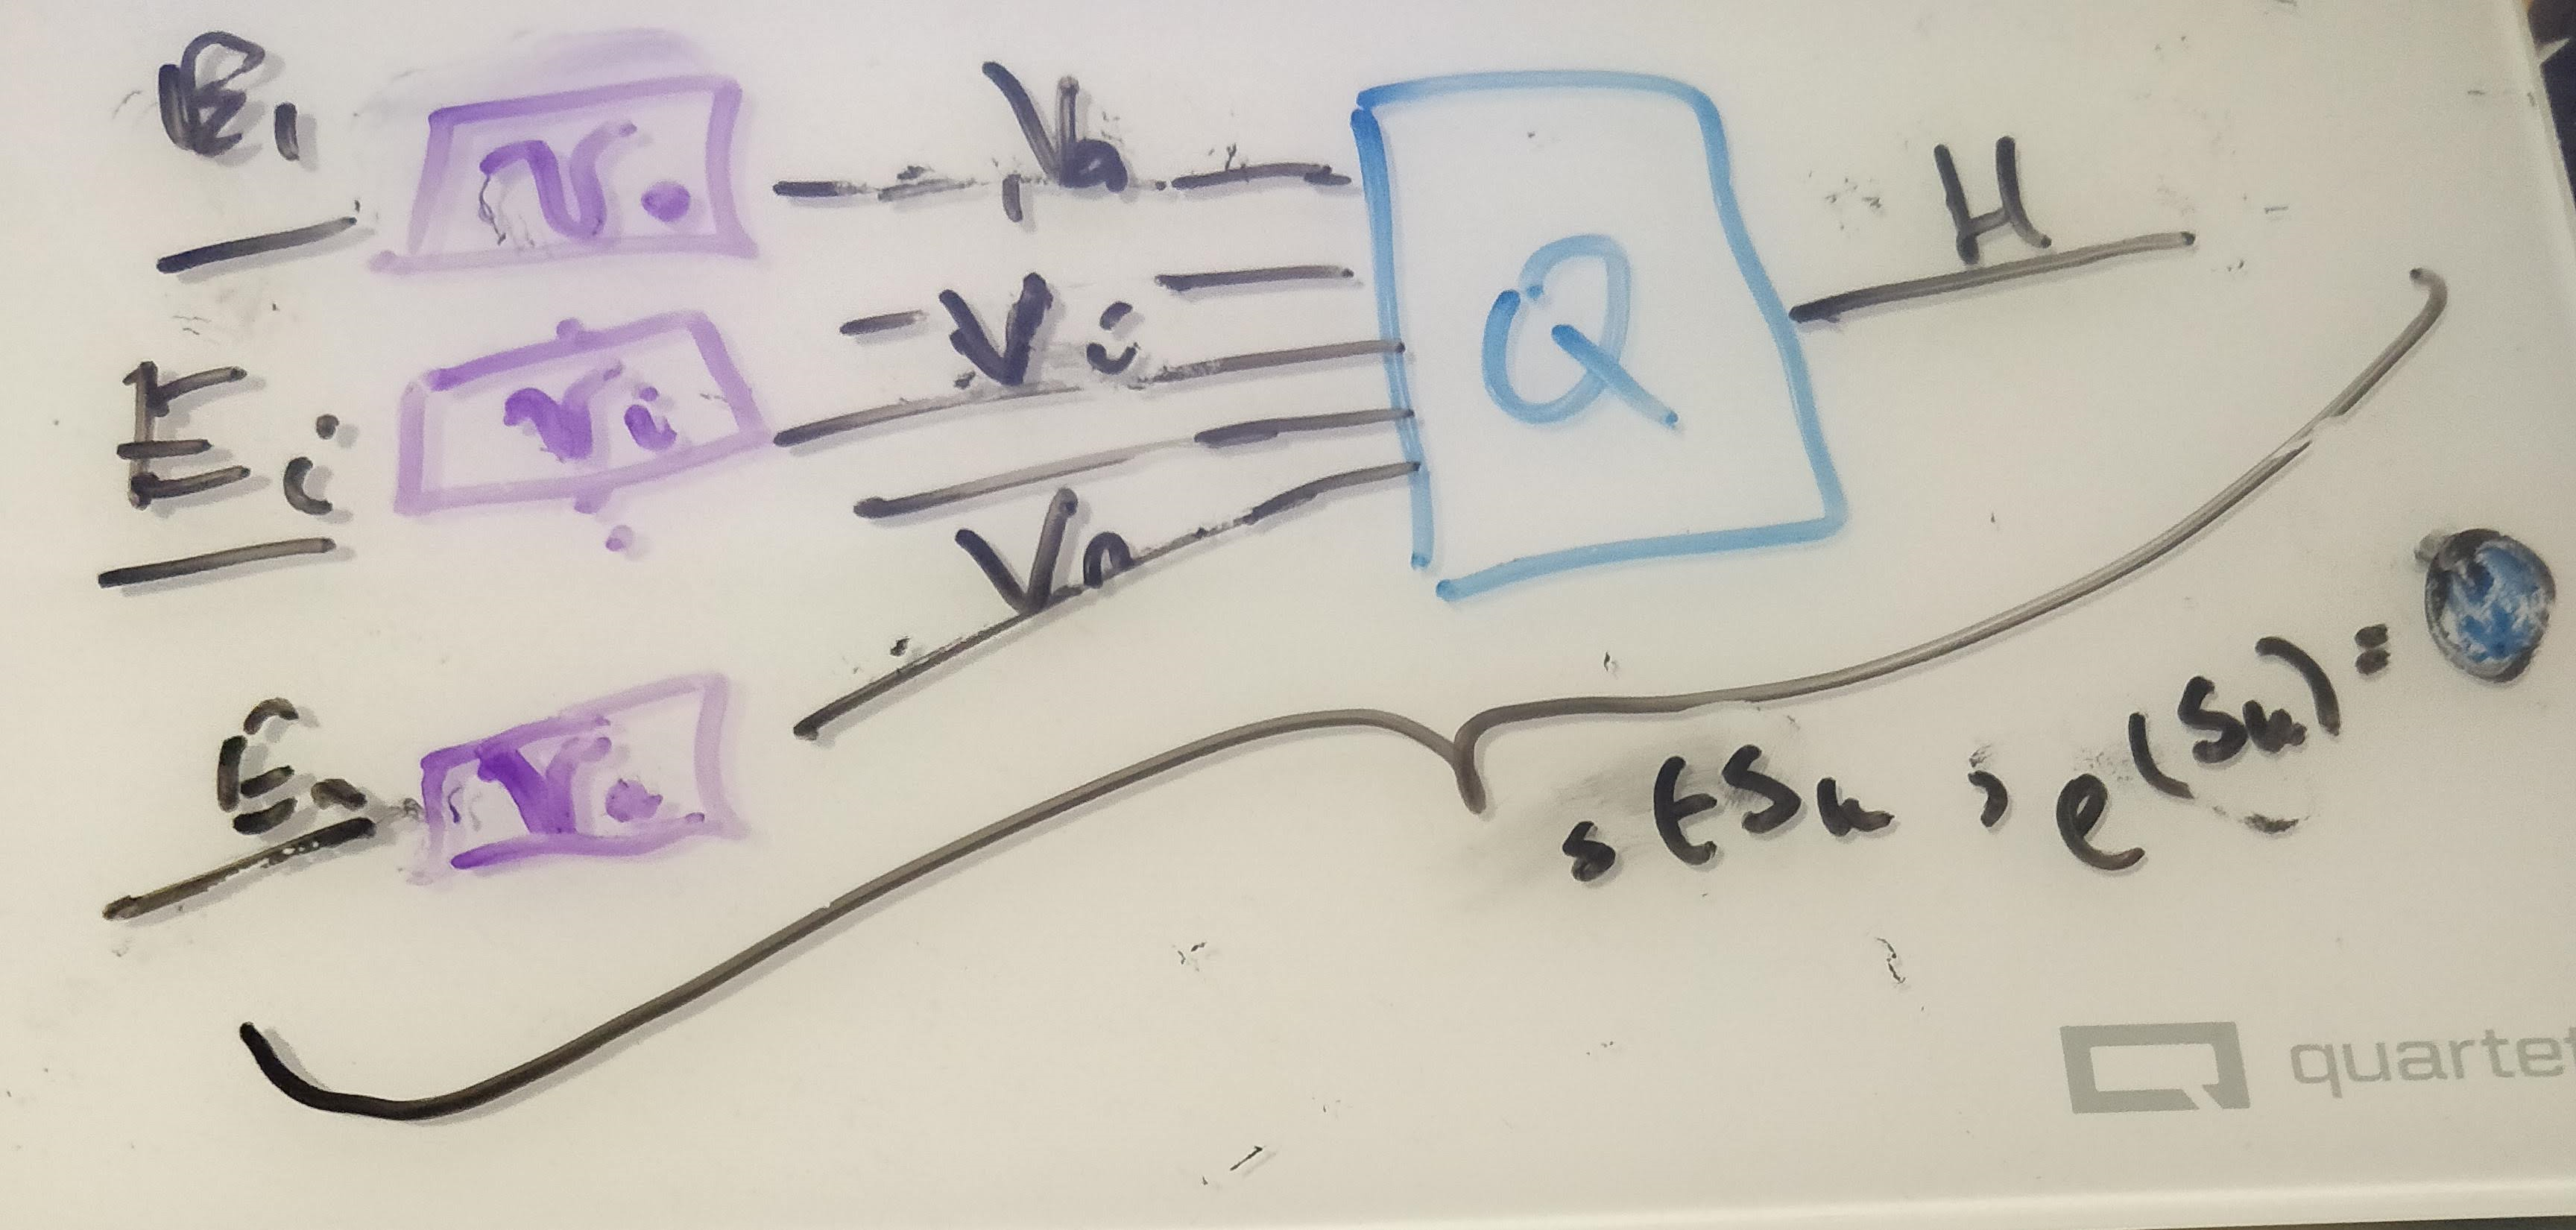
\includegraphics[width=\textwidth]{figures/sections/math/path_of_q}
    \label{fig:artist_q}
    \caption{The $\nu$ functions convert data $E$ to visual $V$. $Q$ assembles the different types of visual parameters $V_{i}$ into a graphic in $H$. $Q\circ\mu(\xi^{-1}J)$ forms a visual mark by applying $Q$ to a region mapped to connected components $J \subset K$.}  
\end{figure}

As shown in figure~\ref{fig:artist_q}, $Q$ takes the individual fields in $V$ as input and outputs a single piece of a graphic on $H$. As with $\nu$, the constraint on $Q$ is that for every monoid actions on the input in $V$ there is a corresponding monoid action on the output in $H$:
\begin{equation}
    Q: \Gamma(V) \rightarrow \Gamma(H)
\end{equation}

$Q: \mu \mapsto \rho$

We want a monoid/group action on $Q(\Gamma(V))$, do not need an action on all of $\Gamma(H)$


To output a mark  \cite{bertinIIPropertiesGraphic2011,carpendaleVisualRepresentationSemiology}, $Q$ is called with all the regions $s$ that map back to a set of connected components $J \subset K$:
\begin{equation}
J = \{j \in K \text{ s. t. } \exists \gamma \text{ s.t. } \gamma(0)=k \text{ and }\gamma(1)=j\}
\end{equation}
where the path\cite{ConnectedSpace2020}  $\gamma$ from $k$ to $j$ is a continous function from the interval [0,1].

We define the mark as the graphic generated by $Q(S_j)$:

\begin{equation}
    \begin{tikzcd}
        H \arrow[r, shift left] & S_j \arrow[rr, "\xi(s)", shift left] \arrow[l, "\rho(S_j)"] &  & J_{k} \arrow[ll, "\xi^{-1}(J)"]
        \end{tikzcd}
    \label{eq:mark}
\end{equation}

where the set $j \subset J$ is the set of marks in the graphic.

$M = M_{1} \times M_{2} \times \ldots \times M_{n}$
color X xpos (Cross product of monoid actions over V/E), cartesian product b/c independent. $M$ over $E$ was translated to acting over $\Gamma(V)$ of these act on $\Gamma(V)$
$\nu$ translates the sets, constraint on $\nu$ is equivariance of M. Is limited to the $Q(\Gamma(V))\subset of \Gamma(H)$ because not all visual tramsforms ($\mu$) are supported by all  $\rho$.

\begin{figure}
    \includegraphics[width=\textwidth]{figures/sections/math/diff_type_q.png}
\end{figure}
So we define the actions $M$ on the image of $Q$, $Q(\Gamma(V)) = Y$. We can backward define our actions?

When the visual atrtribute in $\mu$ is some kind of direct property of D, then we can define $M$ on $\Gamma(H)$ and require that $Q$ preserves it. But we have graphical parameters that do not apply to the whole glyph and therefore are not direct mappings on D, such as facecolor or line thickness. For these types of properties, we need to define an action on the target graphic $Q(\Gamma(V)) \in \Gamma(H)$.
%%in a direct transformation of D, the map on s to d will fall out. Need the eqiuvariance in cases where there are not direct maps to D but instead are partial/compositional/ 

If can check this on $Q$, then you can define an equivariant $M$. Use action of $M$ on $V$ to define action $M$ on $Y$. 

Let ....

If $\forall g \in M$ and $\forall \mu, \mu\prime \in X$, 
\begin{equation}
Q(\mu) = Q(x2) 
\end{equation}
If true, then we can define a group action on $Y$ is defined as $g\circ \rho = \rho\prime$ where $\rho\prime=Q(g\circ \mu)$ with $\mu \in Q^{-1}(\rho)$.

tuple of figure above Is ... %%mu is first circle, mu' is second circle, broken mu is squggle%%
if two $\mu$ go to the same graphic(glyph), then if we transform them the same way they need to generate the same graphic in H. two sections of V if they map to the same thing, they need to map to the same thing if you transform they need to map to the same thing. 

change g to  m

%% m is a cartesian product of group actions in M, for example {identity, ...., identity, thickens}
%% \mu and \mu' are different sections of \Gamma(V)

\paragraph{Example: Invalid Q}
Check a well defined map $M\times Y \rightarrow Y$.


constraint: inputs go to same output means changes to inputs mean same changes to output

\subsubsection{Visual Idioms: Equivalance class of artists}
Given $O(E)$ of the same type that output to the same type of graphic $O(H)$, the 


Natural transformation + composition is partial ordering? Back and forth is equivalent 
\end{document}